%!TEX root = ..\..\dissertation.tex
\chapter{Introduction}\label{chp:Introduction}
%Why is the topic of interest?
% \todo[inline]{Intro 07/06}
At the threshold of the fourth industrial revolution, an era of increased digitalisation, variety, and personalisation in manufacturing is at hand.
Manufacturers are presented with countless new opportunities and challenges.
Their ability to remain competitive is critically dependent on managing these changes within the industry---a task that has proven momentous for many companies~\parencite{ElMaraghy2013629}.

%Defining manufacturing systems
At its core, manufacture in an industrial setting is the making or producing of wares, goods, and products from one or more other materials or parts through manufacturing processes.
These manufacturing processes change (or transform) the original product or material in a number of ways, \eg{} by removing material, joining it to another material, or modifying it's properties.
The manufacturing process, or in more general terms the transformation process, is essentially a series of effects carried out on a product or material in its initial state to transform it into a desired state.
A transformation process does not stand on its own, but is part of a \gls{glos:tranSystem} containing also the execution system performing the transformation process, and the active environment influencing the process~\parencite{Hubka88}.
The execution system itself consists of the technical system, containing machinery and tools carrying out the actual transformation process, and the human system, containing any needed human operators for the machinery.
A diagram of the transformation system and its elements is shown on \cref{fig:transfSystem}.
\begin{figure}[tb]
	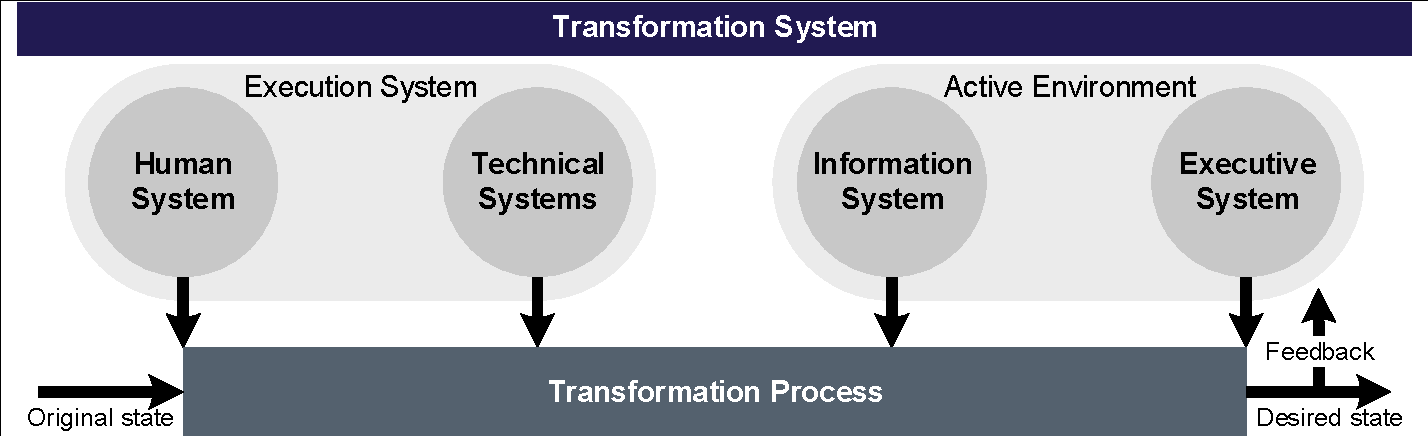
\includegraphics[width=\textwidth, trim=2 2 2 2, clip]{mainmatter/introduction/figures/TTS.pdf}
	\caption[Diagram of the transformation system.]
	{Diagram of the transformation system, adapted from~\textcite{Hubka88}.
	The active environment also includes influences outside the trasnformation system itself such as time and space (not pictured).
	The executive system can also be considered the management and goal system, while the information system is a storage medium and source.
	For the sake of simplicity, ecosystems and all factors not included in the human system, technical systems, and transformation process are collected in the active environment.}\label{fig:transfSystem}
\end{figure}

When people speak of manufacturing systems, it is typically the combined human and technical system within the transformation system.
Sometimes, parts or all of the active environment for the manufacturing system are considered part of the system itself.
But such transformation processes and systems exist everywhere and may be both intentional and unintentional, desirable and undesirable in relation to human needs.
So while a manufacturing system can be considered a transformation system, a more precise designation is that of a \gls{glos:techSystem} which, along with a human system, executes technical processes rather than transformation processes.
This distinction is important, since a \gls{glos:techProc} is a specific type of transformation process where humans use technical systems as artificially created tools, while transformation systems also cover naturally occurring phenomenons~\parencite{Hubka88}, \eg{} biological or environmental processes.
Often, the terms production system and manufacturing system are used interchangeably.
This thesis will primarily use the term manufacturing system as described above, \ie{} the technical system, and use the term production in a wider sense, covering the manufacturing system as well as logistics, planning, and control, \ie{} the broader transformation system
% \todo[inline]{Bring in GDP and manufacturing contributions in general}

% \section{On the evolution of manufacturing systems}
One of the earliest and most well-known examples of the modern manufacturing system is the Ford Model-T mass production line, rapidly producing thousands of near-identical cars.
Since before the Ford Model-T, the evolution of manufacturing has been driven by manufacturers seeking to minimise costs while increasing quality, reliability, and profit.
To enable this, and manufacture increasingly complex products, new materials and processing techniques have continuously been introduced, advancing production technology and shaping the manufacturing industry as a whole~\parencite{ElMaraghySmartChange}.
A currently ongoing change is the transition from mass production towards mass customisation and personalisation; a direction that does not seem to be changing soon~\parencite{Salvador_MITSMR}.
The trend towards increasing product variety and shortening product development life cycles is causing a misalignment between products and the manufacturing systems that produce them~\parencite{HodaC}.
Dedicated manufacturing systems, manufacturing only a very limited number of product variants (like the Ford Model-T systems), tend to outlive the life cycles of the product generations they manufacture.
As a result of the increased demand for variety, manufacturing systems must be able to manufacture multiple generations and variants of products, pushing manufacturers in the direction of changeable manufacturing, \eg{} flexible, reconfigurable manufacturing systems~\parencite{WIENDAHL2007783,ElMaraghy2013629}---a manufacturing paradigm shift, as illustrated on \cref{fig:evoMfgPara}.
Manufacturing systems and the industry itself will continue to evolve.
\begin{figure}[tb]
	\centering
	\makebox[\textwidth][c]{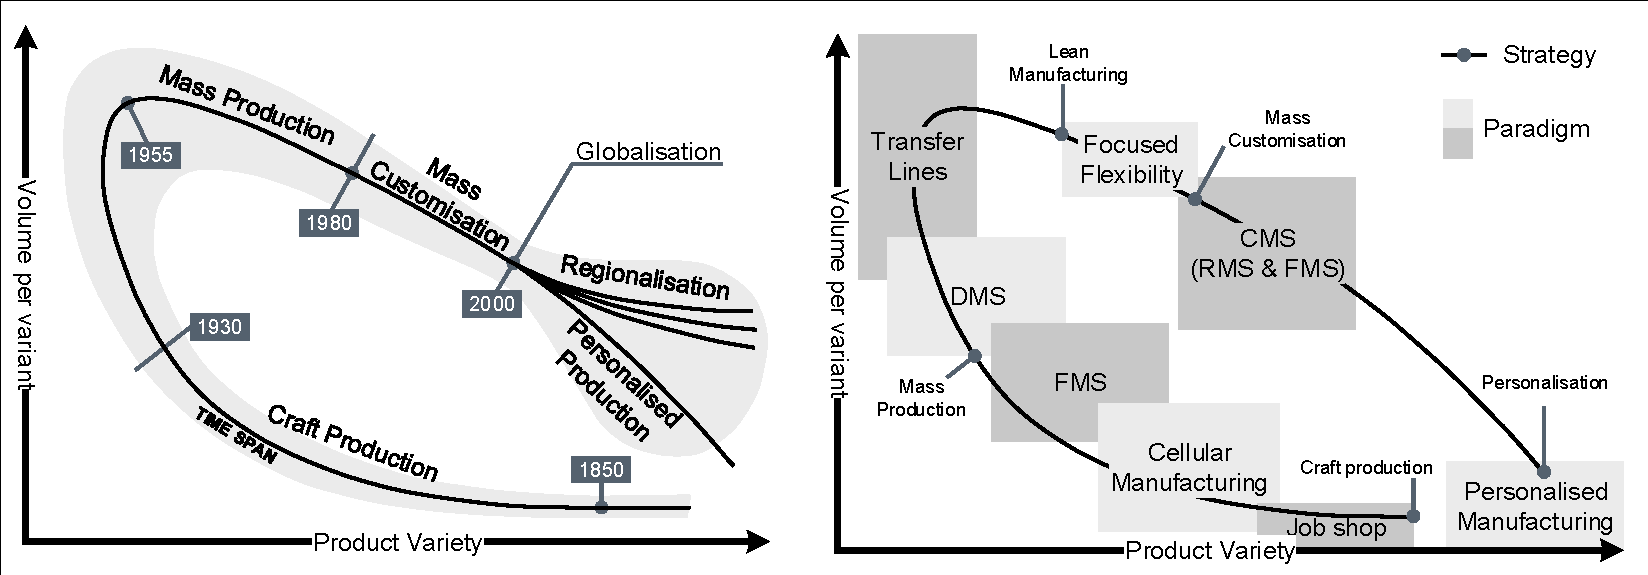
\includegraphics[width=1.1\textwidth, trim=2 2 2 2, clip]{mainmatter/introduction/figures/mfgParaEvo.pdf}}
	\caption[Evolution of the manufacturing and manufacturing system paradigms.]
	{Left: Evolution of the manufacturing paradigm, from craft production to mass production, mass customisation and mass personalisation.
	Adapted from \textcite{KorenGlobalManRev}.
	Right: Evolution of the manufacturing systems paradigms.
	Adapted from \textcite{ElMaraghy2013629}.
	FMS (Flexible Manufacturing System), DMS (Dedicated Manufacturing System), \gls{glos:CMS} (Changeable Manufacturing System), \gls{glos:RMS} (Reconfigurable Manufacturing System).}\label{fig:evoMfgPara}
\end{figure}

%I4.0, IoT, IIoT, IoP, big data etc.
Amidst the fourth industrial revolution heading towards Industry 4.0, enabling technologies are also evolving and advancing.
To mention a few, information processing speeds are becoming faster, sensors are becoming more sophisticated, machine learning and artificial intelligence are gaining ground, all while technology costs and availability are improving.
All of these and more are leading to more available data and more sophisticated analysis supporting effective and efficient decision-making in manufacturing companies.
These advances in technology enable improved communication both between systems within a company and elements of individual systems, leading to increased digitalisation, data exchange, and analytics~\parencite{Jeschke2017}.
Concepts related to Industry 4.0, such as the Industrial Internet of Things (IIoT) and Internet of Production (IoP), employ these new technologies and strategies to lay the foundation for quicker and more knowledge-based decision-making when it comes to reconfiguring or changing a manufacturing system~\parencite{ElMaraghySmartChange}.

Achieving manufacturing systems capable of reconfiguration and change remains a challenge for many manufacturers.
To address the adversity posed by increasing variety and complications implementing changeable manufacturing, manufacturing system platforms, platform-based co-development, and co-\gls{glos:platforming} are gaining traction in research~\parencite{MichaelisJohannesson,ElMaraghy2015407,ABBAS201851,SorensenMCPC2017}.
The following sections define several terms used throughout this thesis, all of which are summarised in the index on \cpageref{main}. 
They furthermore provide a state-of-the-art for manufacturing system platforms, their background, nature, and connection to related subjects.
Finally, what has been attempted in the present effort is outlined, followed by a description of this thesis' structure.

%What is the background on previous solutions, if any?
%!TEX root = ..\..\dissertation.tex
\section{On Platforms}
Platforms are a way to manage variety by allowing certain areas or features of a product or system to be changed, while standardising and effectively ``locking'' other features. 
They are essentially a collection of decisions on certain aspects of a system, which designers and developers must adhere to when creating a new system.
These decisions can be made for various purposes, \eg{} to ensure compatibility between system generations, speed up the system design process, ensure system robustness, ease integration of new technology, or guarantee manufacturability, to mention a few.
Standardisation of physical and non-physical assets, as well as the sharing of these assets or characteristics, \ie{} \gls{glos:cmmnlty}, is the core of platforms.
In this way, new system variants and generations can relatively quickly be created by designers and developers utilising platforms.
As such, platforms are the result of answering two essential questions with regards to a system~\parencite{SorensenMCPC2017}:
\begin{itemize}
	\item What may change and what may not?
	\item Where is variety acceptable and where is it not?
\end{itemize}
One area where platforms have seen significant success is in product design and development, where they have been successfully adopted to manage an increasing number of product variants~\parencite{AIE:276705}.
While various definitions pertaining to platforms exist, this thesis subscribes to the definition proposed by~\textcite{MeyerLehnerd}.
\begin{definition}{\gls{glos:platform}}
a collection of elements and interfaces forming a common structure, from which a stream of derivative products can be efficiently developed~\parencite{MeyerLehnerd}
\end{definition}
This makes the platform itself distinct from another commonly used term in product design and development; product family.
Where a platform is a collection of entities from which products are built, a product family is a collection of products sharing certain common characteristics, which may have been built on a platform.
The definition above was originally aimed towards products (\ie{} product platforms), but it is also considered pertinent when discussing manufacturing systems, as these are considered the product of a targeted design and development process, and a technical product can generally be considered a system.
Research in the development, implementation, and utilisation of manufacturing system platforms is sparse and examples are few~\parencite{BossenPbCd,SorensenAPMS2018}, but several well-known aspects of product platforms can be applied to manufacturing system platforms as well.
Among these are the core concepts of architecture, modules, interactions, and interfaces.

\subsection{Architecture}
The concept of system \gls{glos:arch} is similar to that of platforms, and the two terms are often used interchangeably despite significant differences between the two.
In system design and development, regardless of whether these systems are products or manufacturing systems, an architecture is essentially a description of a system or system of systems.
It captures both the functional and physical elements of a system, how they relate to each other, and how the system interacts with its environment.
Where a platform contains the standardised elements or features upon which systems can be or are built, the architecture contains all elements and relations of a system, including those that are not standardised~\parencite{HarlouU}.
As such, a platform can be considered a subset of an architecture.
However, while all systems exhibit an architecture (explicit and intentionally developed or otherwise), not all systems exhibit platforms.
Architectures are commonly used within systems engineering and software development~\parencite{9781118999400,ISO42010}.
This thesis aligns itself with a slightly modified definition of architecture by \textcite{UlrichEppinger}, relying on the notion of modules discussed in the following section.
\begin{definition}{\gls{glos:arch}}
the architecture of a system is the scheme by which the functional elements of the system are arranged into modules and by which the modules interact
\end{definition}

\subsection{Modules}
Platforms and modules are closely related, but remain distinct concepts~\parencite{DitlevModDrivers}.
A module is an entity designed to implement one or more well-defined functions, with well-defined interfaces connecting one module to another.
Examples of various common types of modularity are shown on \cref{fig:typesModularity}.
\begin{figure}[tb]
	\centering
	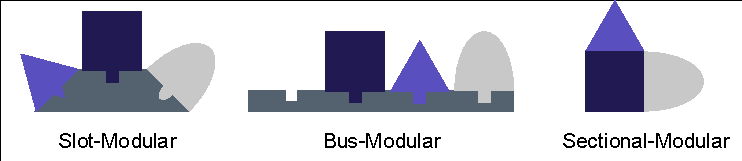
\includegraphics[width=.8\textwidth, trim=3 3 3 3, clip]{mainmatter/introduction/figures/modularity.pdf}
	\caption[Three common types of modularity.]
	{Three common types of modularity.
	Redrawn from \textcite{UlrichEppinger}.}\label{fig:typesModularity}
\end{figure}
This aligns with the core purposes of a platform, since modules are essentially standardised assets, functions, and interfaces.
Platforms are characterised by a particular type of modularity, as the constituents of a platform are elements with low variety and high reusability~\parencite{BaldwinWoodard2009}, making platforms modular by nature.
Systems based on platforms will typically be constructed from these platform modules of low variety and high reusability, combined with a number of modules with high variety and low reusability in order to create the desired variety of the system.
There can be a number of reasons for why a module exists or why a particular set of functions are encapsulated in a single module.
These are generally dubbed module drivers, and represent different criteria behind modularisation~\parencite{Erixon19961}.
Although the module drivers were originally defined for product design and development, \textcite{DitlevModDrivers} identified several drivers applicable within production and manufacturing system design, as outlined in \cref{tab:modularDrivers}.
\begin{table}
	\centering
	\caption[Relevant drivers for modular production.]
	{Relevant drivers for modular production.
	Adapted from \parencite{DitlevModDrivers}.}\label{tab:modularDrivers}
	\small
	\begin{tabular}{p{.16\textwidth}p{.27\textwidth}p{.4\textwidth}}
		\toprule
		Category & Driver & Description\\
		\midrule
		\multirow{3}{.2\textwidth}{System Development} & Geometric Integration and Precision & Careful alignment of parts and manufacturing assets.\\
		& Function Sharing & Two or more manufacturing assets sharing a common function.\\
		& Portability of Interfaces & Ease of connecting two manufacturing assets via an interface.\\
		\midrule
		\multirow{3}{.2\textwidth}{Localization of Changes} & Module Carryover & Functions not expected to change in the future.\\
		& Technology Evolution & Changes expected due to implementation of new manufacturing technology.\\
		& Planned Product Changes & Planned changes due to product/production planning.\\
		\midrule
		\multirow{2}{.2\textwidth}{Variety and Standardisation} & Common Unit & Function required by several different manufacturing assets.\\
		& Different Specification & Function required for localised differentiation.\\
		\midrule
		Production of Manufacturing equipment & Vendor Capabilities & Outsourced functions.\\
		\midrule
		Service and Recycling & Service and Maintenance & Frequently used functions subject to wear.\\
		\bottomrule
	\end{tabular}
\end{table}


\subsection{Interfaces \& Interactions}
To describe how systems and their elements interact and are influenced by each other and the environment, the terms interaction and interface will be used.
An \gls{glos:interaction} is some effect that occurs between at least two objects, while an \gls{glos:interface} is how said effect is transferred from one object to another.
The distinction between these two is often overlooked, as the focus is typically on interfaces, which tend to cover both terms in one.
It is, however, an important distinction to make when it comes to platform development in order to identify similar interactions carried out over different interfaces.
\begin{definition}{\gls{glos:interaction}}
a mutual or reciprocal action occurring as a result of two or more objects influencing each other
\end{definition}
\begin{definition}{\gls{glos:interface}}
a point of contact between two or more objects, at and/or through which an interaction occurs
\end{definition}

Interactions are further classified into four generic types; spatial, energy, information, and material~\parencite{Pimmler94integrationanalysis}.
A spatial interaction calls for adjacency, orientation, or alignment, \eg{} two parts oriented for assembly, or a gripper being adjacent to the end of an articulated robot.
An energy interaction describes a need for energy transfer, \eg{} the transfer of heat from a processor to a heatsink, or power from a power supply to components in a control system.
An information interaction identifies a need for information, data, or signal exchange, \eg{} exchange of information between a sensor and a control system or processor.
A material interaction calls for material exchange, \eg{} airflow over a heatsink or water from a pump to a pipe system.
Individual interfaces can facilitate multiple interactions depending on the level of detail being considered.
In the case of the interaction between the heatsink and processor described above, there is also a need for a physical contact and alignment (\ie{} a spatial interaction) between the two components.
Such interactions between heatsink and processor can be realised in various manners.
Screws and pins can be used to align the two components, while a thermal interface material (such as cooling paste) can be used to facilitate the transfer of heat and absorb tolerances from spatial alignment.
Fans attached to the heatsink can then provide an increased airflow for a material interaction, and the processor can be connected to a sensor and power supply through wires or pins on a motherboard for energy, information, and spatial interactions.

\subsection{Manufacturing System Platforms and Changeable Manufacturing}\label{ssec:pPlatforms}
Development and utilisation of platforms in manufacturing is an enabler for changeable manufacturing; a way to improve variety management in manufacturing systems.
Changeable manufacturing is a manufacturing paradigm based on the concept of \gls{glos:changeability}, \ie{} the characteristics giving manufacturing systems the capability to accommodate to change in an economical manner by making adjustments at all levels of a factory~\parencite{HodaC}.
It is an umbrella term encapsulating a number of so-called \gls{glos:changeability} classes, each relating to specific levels within a factory, as shown on~\cref{fig:chngbltyClasses}.
Each level, when broken down, consists of one or more instances on the lower level, \eg{} a network consisting of multiple factories, a factory consisting of multiple segments, and a segment consisting of multiple manufacturing systems.
\begin{figure}[tb]
	\centering
	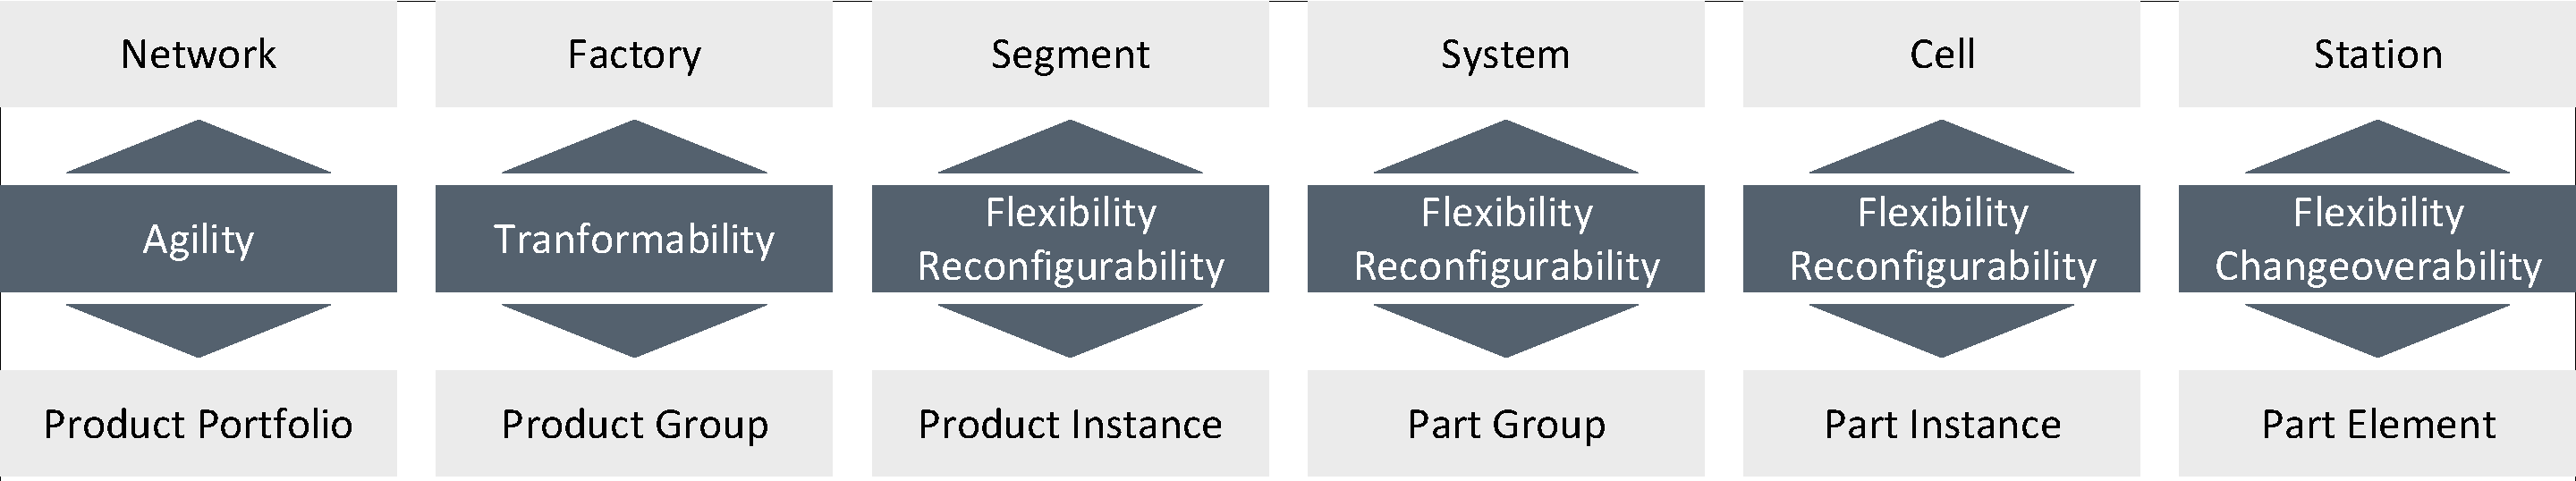
\includegraphics[width=\textwidth, trim=3 3 3 3, clip]{mainmatter/introduction/figures/factoryLevels.pdf}
	\caption[The six levels of a factory, their corresponding changeability class and equivalent product level.]
	{The six levels of a factory (top), with their corresponding changeability class (mid), and the equivalent product level (bottom).
	Adopted from \textcite{HodaC}.}\label{fig:chngbltyClasses}
\end{figure}
The five changeability classes are briefly outlined below~\parencite{HodaC}:
\begin{itemize}
	\item \textbf{Agility:} strategic ability of a company to respond to volatile market conditions, \eg{} by pursuing new markets, services, products, or manufacturing systems.
	\item \textbf{Transformability:} tactical ability of a factory to switch between a variety of product groups or families.
	\item \textbf{\Gls{glos:reconf}:} ability of a production area to, through a physical change, switch between similar product groups or families with relative ease and speed.
	\item \textbf{Flexibility:} operative ability of a production system to, without a physical change, switch between variants within a predefined product family quickly and effortlessly.
	\item \textbf{Changeoverability:} operative ability of a workstation to perform specific operations without effort and delay.
\end{itemize}
Traditional dedicated manufacturing systems (DMS), lacking the characteristics facilitating change, are unable to keep up with the rapid introduction of new technologies, products, and variants.
Changeable manufacturing systems (\gls{glos:CMS})---\ie{} manufacturing systems possessing characteristics giving them the capability to accommodate change---and in particular reconfigurable manufacturing systems (\gls{glos:RMS}) are becoming increasingly relevant to manufacturers.
One of the key characteristics of \gls{glos:RMS} is modularity~\parencite{Koren,HodaC}.
The modular nature of both platforms and RMS implies a connection between the two.
In fact, the utilisation of platforms to design an RMS can be considered part of the basic and advanced design phases of RMS design.
Following \posscite{Andersen2017179} generic method for RMS design, platforms can play into the basic design phase when realisation of \gls{glos:reconf} and functionality is determined, interfaces identified and specified, and system elements are decided upon.
A simplified illustration of the design approach is shown on \cref{fig:pltfRMS}, with highlights added to illustrate when platforms can provide a benefit.
For the advanced design phase, the platform plays into the detailing of system modules, system interfaces, and detailed manufacturing equipment design.
These functional elements, enablers, interactions, interfaces, and modules are all things a platform should include.
\begin{figure}[tb]
	\centering
	\makebox[\textwidth][c]{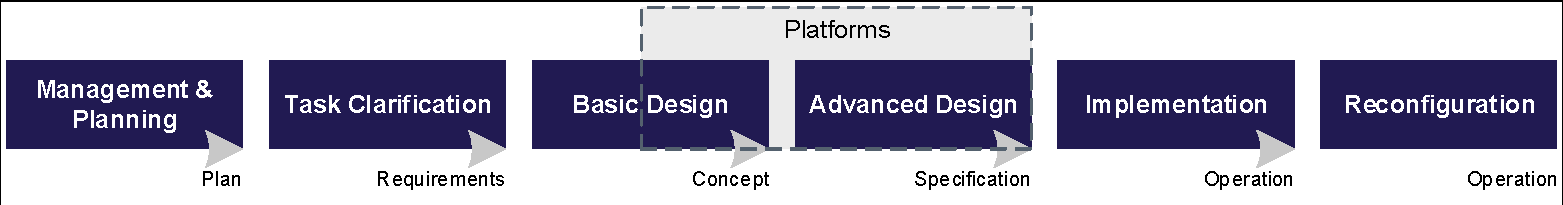
\includegraphics[width=1.1\textwidth, trim=2 2 2 2, clip]{mainmatter/introduction/figures/genericRMS.pdf}}
	\caption[Generic reconfigurable manufacturing system design approach.]
	{Simplified generic reconfigurable manufacturing system design approach by \textcite{Andersen2017179}.
	A dashed box has been highlighted to during which stages utilisation of platforms provide the largest benefit~\parencite{SorensenCMS2019}.}\label{fig:pltfRMS}
\end{figure}

With the development, implementation, and utilisation of manufacturing system platforms remaining a relatively immature field of research, attempts at drawing inspiration, concepts, and methods from other areas where maturity is higher and platforms are more common have previously been made, especially borrowing from software architecture and development~\parencite{SorensenMCPC2017,BENKAMOUN201488,JepsenPhD,BossenCMod}.
Having both a product and manufacturing system platform available could greatly limit the effects of introducing a new product variant or generation, preventing these changes from propagating throughout a manufacturing company.
Utilising both types of platforms in conjunction facilitates co-development of new solutions across departments in a manufacturing company.

%What is the background on potential solutions?
%!TEX root = ..\..\dissertation.tex
\section{Co-Development \& Co-Platforming}\label{sec:coDevPltf}
Co-development in systems engineering, product, and production design refers to the simultaneous development or design of two or more systems with some required or anticipated mutual effect on each other, \eg{} a product and the manufacturing system producing it.
Co-development, along with the related concept co-\gls{glos:platforming}, has been gaining footing in research on platforms and reconfigurable manufacturing in particular~\parencite{MichaelisJohannesson,ElMaraghy2015407}.
The end-goal of co-development of products and manufacturing systems, as outlined by~\textcite{MichaelisJohannesson} and shown on \cref{fig:pltfCoDev}, is to achieve platform-based co-development, wherein aligned instantiations of the platforms are simultaneously created as explicit configurations of products and their corresponding manufacturing system.
\begin{figure}[tb]
	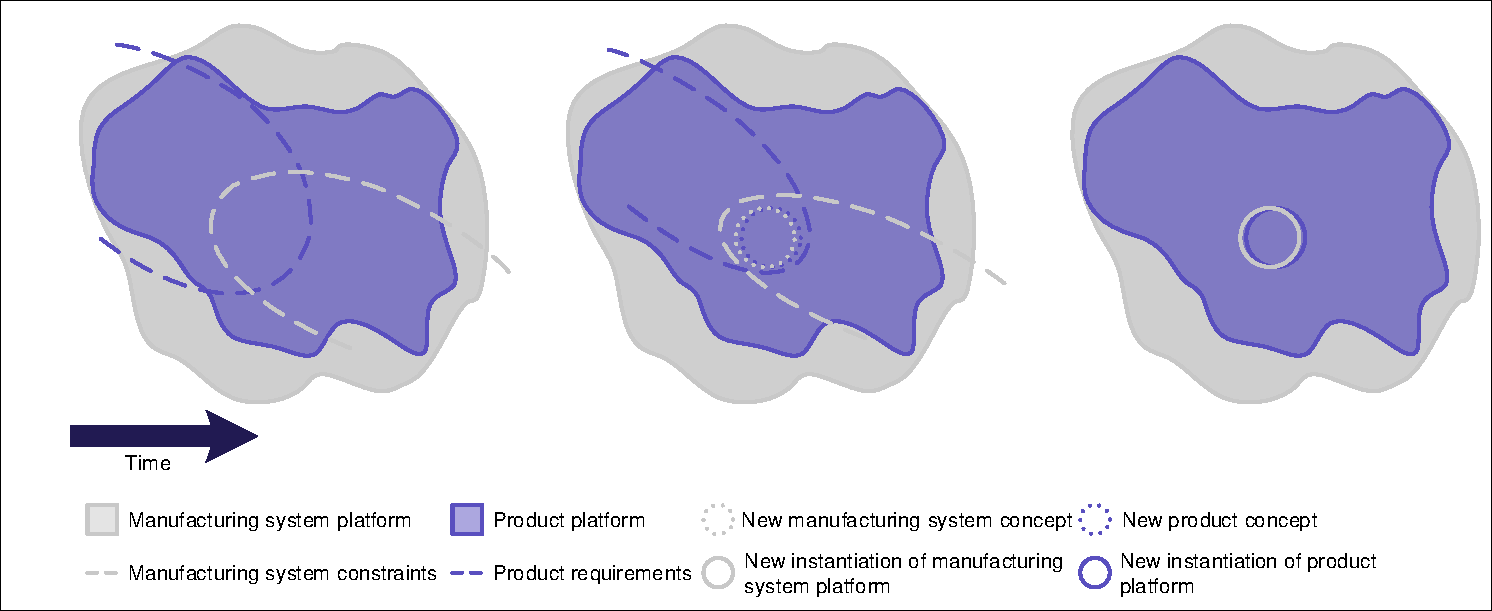
\includegraphics[width=\textwidth, trim=2 2 2 2, clip]{mainmatter/introduction/figures/pltfCoDev.pdf}
	\caption[Platform-based co-development.]
	{Platform-based co-development with new instantiations of the product and manufacturing system platform being developed alongside each other to ensure alignment and compatibility.
	Adapted from \textcite{MichaelisJohannesson}.}\label{fig:pltfCoDev}
\end{figure}

Inconsistencies and lack of communication with regards to platform development as well as misalignment between platforms have proven massive challenges for manufacturers~\parencite{SorensenAPMS2018}.
To address this, and generally improve the synergy between product and manufacturing system development, various approaches to integrate and align the two areas are appearing, such as integrated product and production modelling~\parencite{Michaelis2015203,BRUNOE2018592,BrunoePPModel}, resource modelling and capability matchmaking \parencite{7750724,JARVENPAA201887,dhunganaMarket}, and set-based concurrent engineering utilising platforms \parencite{Levandowski2014,Levandowski01092014,LANDAHL201661}.
Such approaches provide support for a formal way to integrate the work of product and production development teams, ensuring their alignment and compatibility by making it clear which product functions and features are needed, which manufacturing capabilities are available, and how these can be matched, thus facilitating co-development of solutions.

%What was attempted in the present effort?
%!TEX root = ..\..\dissertation.tex
\section{Supporting Independent Development of Platforms}\label{sec:supPltfDev}
In summation, the rising demand for new products, new technologies, and options for personalisation all play a part in increasing the variety manufacturers must be able to handle in order to remain competitive.
Product platforms have successfully been employed to manage this variety in products, but dealing with variety and frequent product changes is straining the capabilities of existing manufacturing systems.
New manufacturing paradigms and the coming fourth industrial revolution present manufacturers with new opportunities to manage variety and improve the capabilities of their manufacturing systems.
Manufacturing system platforms and changeable manufacturing in conjunction with product platforms are seemingly attractive choices to achieve the desired variety and capability of both product and production.

Present effort is a step towards arming manufacturing companies with the necessary background, methods, and tools to independently develop manufacturing system platforms.
Few tools and methods exist aimed explicitly at assisting manufacturers in developing manufacturing system platforms.
Through the studies, projects, and research gathered and presented in this thesis, strides have been made to address this, by gaining inspiration and applying concepts, methods, and tools from various other fields dealing with systems engineering in general.

\subsection{Thesis Structure}\label{sec:thesisStructure}
% What will be presented in this thesis?
This thesis is structured into four chapters and an appendix with six appended papers.
The core purpose and content of each of the four chapters is described below:
\begin{itemize}[font={\normalfont}\bfseries]
  \item[\ref{chp:Introduction}] \textbf{\nameref{chp:Introduction}:}
  Sets the stage for the thesis, introducing its primary subject and context.
  Defines a number of important terms and provides state-of-the-art for manufacturing system platforms, linking it to other relevant research areas.
  \item[\ref{chp:Approach}] \textbf{\nameref{chp:Approach}:}
  Outlines the research approach, covering methodological background and introduces the industrial case.
  Lists research objective, questions and sub-questions addressed through the \PhD{} project.
  \item[\ref{chp:prodPltfDev}] \textbf{\nameref{chp:prodPltfDev}:}
  Describes the contributions made within the research field through the \PhD{} project, based off the six appended papers.
  Provides an extended abstract for each paper and summarises the implications of the contribution.
  \item[\ref{chp:Conclusions}] \textbf{\nameref{chp:Conclusions}:}
  Sums up the main findings of the \PhD{} project and addresses research objectives and questions.
  Discusses findings and applications, and outlines future research.
\end{itemize}